\section*{Ερώτημα 3}
\label{Q3}
\addcontentsline{toc}{section}{\nameref{Q3}}

Έχοντας δημιουργήσει τον μετασχηματισμό Fourier των 4 σημάτων, κατασκευάστηκαν οι παραστάσεις φασματικού περιεχομένουν κάθε σήματος. 

\noindent\\
Είναι γνωστό από την θεωρία πως το σήμα που προκύπτει μέσω μετασχηματισμού Fourier είναι συμμετρικό και έτσι η χρήσιμης πληροφορίας μπορεί να εξαχθεί από το πρώτο μισό του σήματος όμως, για την σωστή αναπαράσταση της συνολικής ενέργειας του σήματος είναι πλέον απαραίτητο να πολλασιαστεί το εξαγόμενο σήμα με το 2. Ακόμα, η χρήσιμη πληροφορία βρίσκεται στο πλάτος του και έτσι μέσω της συνάρτησης abs(), γίνεται υπολογισμός του πλάτους κάθε σήματος.

\noindent\\
Τελικά, τα σήματα που θα χρησιμοποιηθούν για την κατασκευή των γραφικών είναι τα εξής:
\begin{lstlisting}
% Exctracting half of the signal
Y_vol1_h = 2*abs(Y_vol1(1:NFFT/2+1));
Y_vol2_h = 2*abs(Y_vol2(1:NFFT/2+1));
Y_vol3_h = 2*abs(Y_vol3(1:NFFT/2+1));
Y_curr_h = 2*abs(Y_curr(1:NFFT/2+1));
\end{lstlisting}

\subsection*{Τάση εξόδου αντιστροφέα - Voltage\_1}
\label{Q31}
\addcontentsline{toc}{subsection}{\nameref{Q31}}

\noindent
Όσον αφορά το σήμα \textit{Voltage\_1}, αποτελεί το σήμα εξόδου του αντιστροφέα, δηλαδή είναι το AC σήμα που κατασκευάστηκ από το DC σήμα εισόδου. Κατασκευάστηκαν οι γραφικές αναπαραστάσεις του σήματος voltage\_1 στο πεδίο του χρόνου και στο της συχνότητας όπως αυτες φαίνονται στο figure (\ref{Q3_volt1}). Για την καλύτερη απεικόνιση, η γραφική φασματικού περιεχομένου έχει περιοριστεί στα 1000Ηz

\begin{figure}[h]
    \centering
    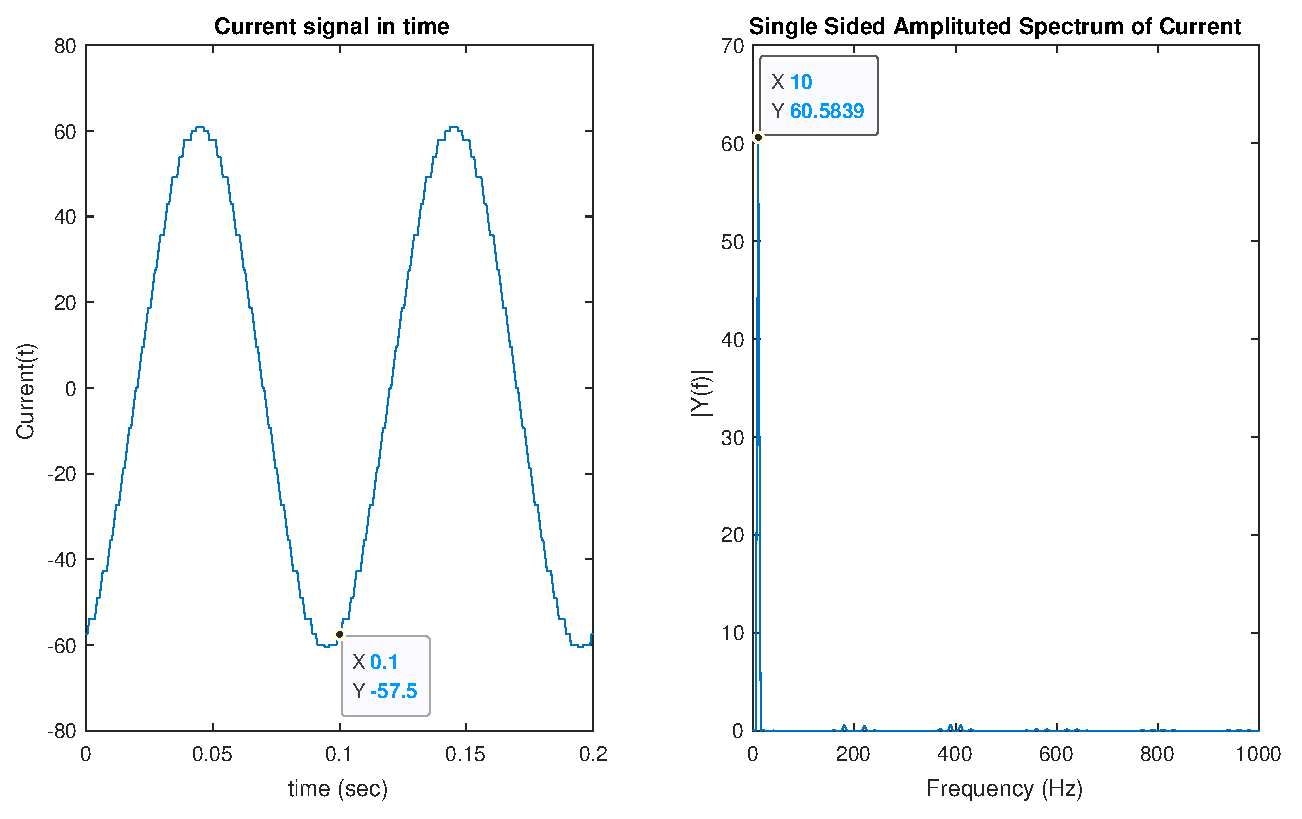
\includegraphics[width=.8\textwidth]{Images/current_Q3.eps}
    \caption{Caption}
    \label{fig:my_label}
\end{figure}

\clearpage
\noindent\\
Όσον αφορά το σήμα του ρεύματος, αρχικά έγινε η γραφική αναπαράσταση του σήματος και του φασματικού περιεχομένου του όπως αυτή φαίνεται στο figure (\ref{}). Για την καλύτερη απεικόνιση, η γραφική φασματικού περιεχομένου έχει περιοριστεί στα 1000Ηz

\begin{figure}[h]
    \centering
    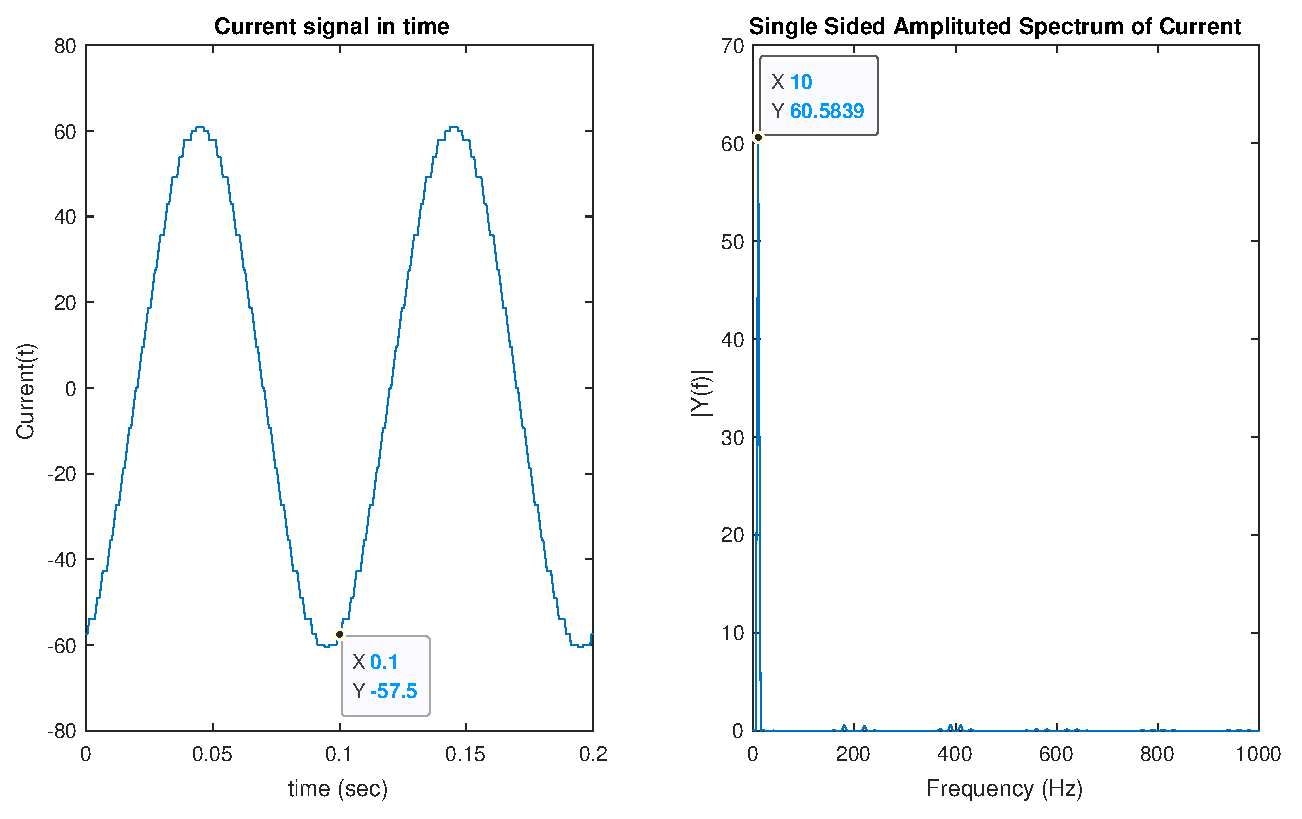
\includegraphics[width=.8\textwidth]{Images/current_Q3.eps}
    \caption{Caption}
    \label{fig:my_label}
\end{figure}

\noindent
Παραπατηρώντας το παραπάνω figure, αρχικά είναι εμφανές πως το σήμα του ρεύματος ομοιάζει αρκετά αυτό του πραγματικού sin(x) και ως αποτέλεσμα αναμένεται να μην παρουσιάζει αρμονικές μεγάλη ισχύς, πέραν της βασικής. Η βασική αρμονική προκύπτει για F = 10Hz κάτι το οποίο είναι αναμενόμενο καθώς η περίοδος του σήματος είναι ίση με 0.1s.

\noindent\\
Εκτός της βασικής αρμονική παρατηρούνται και άλλά μικρά spikes, γύρω από τις συχνότητες 200, 400 και 600 αντίστοιχα, τα οποία οφείλονται στον τρόπο με τον οποίο έχει κατασκευαστεί το σήμα current.